\part{HPC and Exascale}
\chapter*{Introduction}

High Performance Computing, HPC, does not find a strict definition. 
Since computer creation, first dedicated for balistic purposes, domain scientists developped their tool to perform computations. 
Then, in front of the complexity of building such machines, HPC became a dedicated field of research. 

Computer scientists interested in HPC will have to focus on several domains. 
\begin{itemize}
\item The energy consumption, mainly directed by the hardware producers. 
\item The computational power, how to take advantages of the ressources ? 
\item The communication, because such machines are constructed over several machines or nodes. 
\end{itemize}

Domain scientists are also involved directly in HPC with their software and redefining the structure based on their needs and usages. 

%%%%%%%%%%%%%%%%%%%%%%%%%%%%%%%%%%%%%%%%%%%%%%%%%%%%%%%%%%%%%%%%%%%%%
%																	%
%	CHAPTER ONE, THEORY of HPC										%
%																	%
%%%%%%%%%%%%%%%%%%%%%%%%%%%%%%%%%%%%%%%%%%%%%%%%%%%%%%%%%%%%%%%%%%%%%

%%%%%%%%%%%%%%%%%%%%%%%%%%%%%%%%%%%%%%%%%%%%%%%%%%%%%%%%%%%%%%%%%%%%%
%                                                                   %
%	CHAPTER ONE, MODELS of HPC                                       %
%                                                                   %
%%%%%%%%%%%%%%%%%%%%%%%%%%%%%%%%%%%%%%%%%%%%%%%%%%%%%%%%%%%%%%%%%%%%%

\chapter{Models of HPC}

\section{Introduction}

High Performance Computing (HPC) takes his roots from the beginning of computer odyssey in the middle of 20th century.
A lot of rules, observations, theories emerged from it and even Computer Sciences fields. 
In order to understand and characterize HPC and supercomputers, some knowledge on theory is required. 
This part describes the Von Neumann model, the generic model of sequential computer on which every nowadays machine is built.
It is presented along with the Flynn taxonomy that is a classification of the different execution models. 
We also present the different memory models based on those elements. 

Then we give more details on what is parallelism and how to reach performances though it. 
And thus we define what performance implies in HPC. 
The Amdahl's and Gustafson's laws are presented and detailed along with the strong and weak scaling used in our study. 

\section{Von Neumann Model}
\index{Von Neumann Model}
First computers, in early 20th, were built using vacuum tubes making them high power consuming, hard to maintain and expansive to build.
The most famous of first vacuum tubes supercomputers, the ENIAC, was based on decimal system.
It might be the most known of first supercomputers but the real revolution came from its successor.
In 1944 the first binary system based computer, called the Electric Discrete Variable Automatic Computer (EDVAC), was created. 
In the EDVAC team, a physicists described the logical model of this computer and provides a model on which every nowadays computing device is based. 

\begin{figure}
\centering 
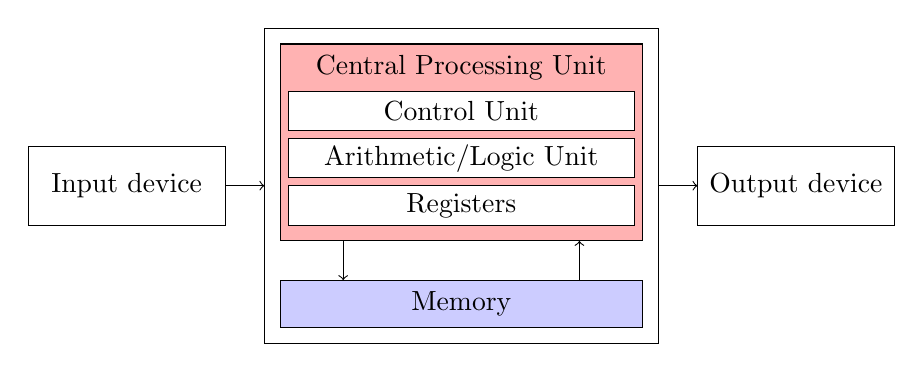
\begin{tikzpicture}
\draw (3,0) rectangle (8,4);
\draw (3.2,1.3) [fill=red!30] rectangle (7.8,3.8);
\node at (5.5,3.5) {Central Processing Unit};

\draw (3.3,1.5) [fill=white] rectangle (7.7,2.) node[pos=.5] {Registers};
\draw (3.3,2.1) [fill=white] rectangle (7.7,2.6) node[pos=.5] {Arithmetic/Logic Unit};
\draw (3.3,2.7) [fill=white] rectangle (7.7,3.2) node[pos=.5] {Control Unit};

\draw (0,1.5) rectangle (2.5,2.5) node[pos=.5] {Input device};
\draw (8.5,1.5) rectangle (11,2.5) node[pos=.5] {Output device};
\draw [->] (2.5,2) -- (3,2);
\draw [->] (8,2) -- (8.5,2);

\draw (3.2,.2) [fill=blue!20] rectangle (7.8,.8) node[pos=.5] {Memory};
\draw [->] (4,1.3) -- (4,.8);
\draw [->] (7,.8) -- (7,1.3);
\end{tikzpicture}
\caption{Von Neumann model}
\label{fig:1_HPC:von_neumann_model}
\end{figure}

John Von Neumann published its \textit{First Draft of a Report on the EDVAC}~\cite{von1993first} in 1945. 
Extracted from this work, the model know as the Von Neumann model or more generally Von Neumann Machine appears. 
The model is presented on figure~\ref{fig:1_HPC:von_neumann_model}.

On that figure we identify three parts, the input and output devices and in the middle the computational device itself. 
\paragraph{Input/Output devices}
The input and output devices are used to store in a read/write way data. 
They can be represented as hard drives, solid state drives, monitors, printers or even mouse and keyboard.
The input and output devices can also be the same, reading and writing in the same area.\\

Inside the computational device we find the memory, for the most common nowadays architectures it can be considered as a Random Access Memory (RAM). 
Several kind of memory exists and will be discussed later. 

\paragraph{Central Processing Unit}
\index{Central Processing Unit}
The Central Processing Unit, CPU, is composed of several elements in this model. 
On one hand, the \textit{Arithmetic and Logic Unit}, ALU, which takes as input one or two values and apply an operation on those data. 
They can be either logics with operations such as AND, OR, XOR, etc. or arithmetics with operations such as ADD, MUL, SUB, etc. 
Of course those operations are way more complex on modern CPUs. 
On the other hand, we find the \textit{Control Unit}, CU, which control the data carriage to the ALU from the memory and the operation to be perform on data.
It is also the part that takes care of the Program Counter (PC), the address of the next instruction in the program. 
We can also identify the Register section which represent data location used for both ALU and CU to store temporary results, the current instruction address, etc. 
Some representation may vary, the Registers can be represented directly inside the ALU or the CU. 
\paragraph{Buses}
The links between those elements are called Buses and can be separated between data buses, control buses and addresses buses.
They will have a huge importance for the first machine optimization, growing the size of the buses from 2, 8, 16, 32, 64 and even more for vector machine with 128 and 256 bits.\\

The usual processing flow on such an architecture can be summarized as a loop: 
\begin{itemize}[noitemsep,nolistsep]
\item[-] Fetch instruction at current PC from memory;
\item[-] Decode instruction using the Instruction Set Architecture (ISA). Known ISA are Reduce Instruction Set Computer architecture (RISC) and Complex Instruction Set Computer architecture (CISC);
\item[-] Evaluate operand(s) address(es);
\item[-] Fetch operand(s) from memory;
\item[-] Execute operation(s), with some instructions sets and new architectures several similar operations can be processed in the same clock time;
\item[-] Store results, increase PC.\\
\end{itemize}

Every devices or machines we describe in the next chapter have this architecture as a basis. 
One will consider execution models and architecture models to characterize HPC architectures.

\section{Flynn taxonomy and execution models}
\index{Flynn taxonomy}
The Von Neumann model gives us a generic idea of how a computational unit is fashioned. 
The constant demand in more powerful computers required the scientists to find more way to provide this computational power.
In 2001, IBM proposed the first multi-core processor on the same die, the Power4 with its 2 cores.
This evolution required new paradigms.
A right characterization is then essential to be able to target the right architecture for the right purpose. 
The Flynn taxonomy presents a hierarchical organization of computation machines and executions models.

\begin{table}
\centering
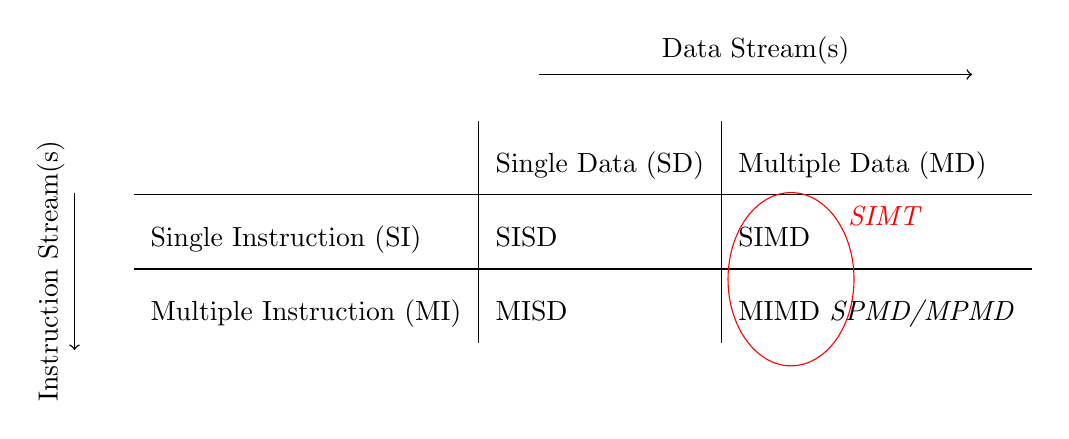
\begin{tikzpicture}
\node (table) {\arraycolsep=1.4pt\def\arraystretch{2.2}
\begin{tabular}{l | l | l}
 & Single Data (SD) & Multiple Data (MD) \\
 \hline 
Single Instruction (SI) & SISD & SIMD \\
\hline 
Multiple Instruction (MI) & MISD & MIMD \textit{SPMD/MPMD} \\
\end{tabular}
};
\draw [->,line width=.5pt] (-0.5,2) -- (5,2) node[midway, above] {Data Stream(s)};
\draw [->,line width=.5pt] (-6.4,0.5) -- (-6.4,-1.5) node[rotate=180,sloped, midway, above] {Instruction Stream(s)};
\draw [red] (2.7,-.6) ellipse (.8cm and 1.1cm) node[xshift=1.2cm,yshift=.8cm] {\textit{SIMT}};
%\draw[decoration={brace,raise=5pt},line width=1pt,decorate]
%  (5,0.4) -- node[right=6pt,yshift=5pt] {\textit{SIMT}} (5,-1.5);
\end{tikzpicture}
\caption{Flynn taxonomy for execution models completed with SPMD and SIMT models}
\label{tab:1_HPC:taxonomy_flynn}
\end{table}

\begin{figure}
\resizebox {.24\columnwidth} {!} {
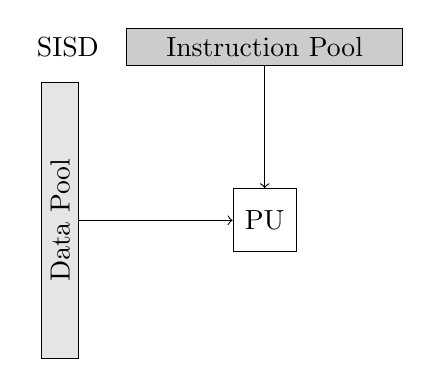
\begin{tikzpicture}
\draw (0.1,5.2) node {SISD}; 
\node (rect) at (2.6,5.2) [draw,minimum width=3.5cm,fill=black!20] (ip) {Instruction Pool};
\node (rect) at (0,3) [rotate=90,draw,minimum width=3.5cm,fill=black!10] (dp) {Data Pool};
\node (rect) at (2.6,3) [draw,minimum width=.8cm,minimum height=.8cm] (pu1) {PU};
\draw [->] (ip) -- (pu1);
\draw [->] (dp) -- (pu1);
\end{tikzpicture}
}
\resizebox {.24\columnwidth} {!} {
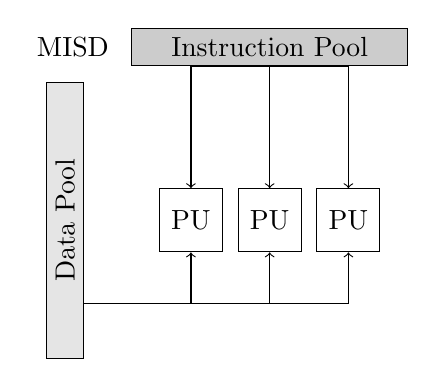
\begin{tikzpicture}
\draw (0.1,5.2) node {MISD}; 
\node (rect) at (2.6,5.2) [draw,minimum width=3.5cm,fill=black!20] (ip) {Instruction Pool};
\node (rect) at (0,3) [rotate=90,draw,minimum width=3.5cm,fill=black!10] (dp) {Data Pool};
\node (rect) at (1.6,3) [draw,minimum width=.8cm,minimum height=.8cm] (pu1) {PU};
\node (rect) at (3.6,3) [draw,minimum width=.8cm,minimum height=.8cm] (pu2) {PU};
\node (rect) at (2.6,3) [draw,minimum width=.8cm,minimum height=.8cm] (pu3) {PU};

\draw[<-] (pu1.north) |-  (ip.south); 
\draw[<-] (pu2.north) |-  (ip.south);
\draw[<-] (pu3.north) |-  (ip.south);

\draw[<-]  (pu1.south) |- ([yshift=-30pt]dp.south);
\draw[<-]  (pu2.south) |- ([yshift=-30pt]dp.south);
\draw[<-]  (pu3.south) |- ([yshift=-30pt]dp.south);

\end{tikzpicture}
}
\resizebox {.24\columnwidth} {!} {
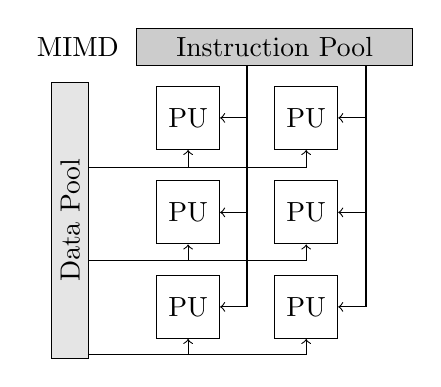
\begin{tikzpicture}
\draw (0.1,5.2) node {MIMD}; 
\node (rect) at (2.6,5.2) [draw,minimum width=3.5cm,fill=black!20] (ip) {Instruction Pool};
\node (rect) at (0,3) [rotate=90,draw,minimum width=3.5cm,fill=black!10] (dp) {Data Pool};
\node (rect) at (1.5,4.3) [draw,minimum width=.8cm,minimum height=.8cm] (pu1) {PU};
\node (rect) at (1.5,3.1) [draw,minimum width=.8cm,minimum height=.8cm] (pu2) {PU};
\node (rect) at (1.5,1.9) [draw,minimum width=.8cm,minimum height=.8cm] (pu3) {PU};
\node (rect) at (3,4.3) [draw,minimum width=.8cm,minimum height=.8cm] (pu4) {PU};
\node (rect) at (3,3.1) [draw,minimum width=.8cm,minimum height=.8cm] (pu5) {PU};
\node (rect) at (3,1.9) [draw,minimum width=.8cm,minimum height=.8cm] (pu6) {PU};

\draw[<-]  (pu1.south) |- ([yshift=19pt]dp.south);
\draw[<-]  (pu4.south) |- ([yshift=19pt]dp.south);

\draw[<-]  (pu2.south) |- ([yshift=-14.5pt]dp.south);
\draw[<-]  (pu5.south) |- ([yshift=-14.5pt]dp.south);

\draw[<-]  (pu3.south) |- ([yshift=-48.5pt]dp.south);
\draw[<-]  (pu6.south) |- ([yshift=-48.5pt]dp.south);

\draw[->] ([xshift=-10pt]ip.south) |- (pu1.east);
\draw[->] ([xshift=-10pt]ip.south) |- (pu2.east);
\draw[->] ([xshift=-10pt]ip.south) |- (pu3.east);

\draw[->] ([xshift=33pt]ip.south) |- (pu4.east);
\draw[->] ([xshift=33pt]ip.south) |- (pu5.east);
\draw[->] ([xshift=33pt]ip.south) |- (pu6.east);

%\draw[<-]  (pu2.south) |- ([yshift=-30pt]dp.south);
%\draw[<-]  (pu3.south) |- ([yshift=-30pt]dp.south);

%\draw [->] (ip) -- (pu1);
%\draw [->] (dp) -- (pu1);
\end{tikzpicture}
}
\resizebox {.24\columnwidth} {!} {
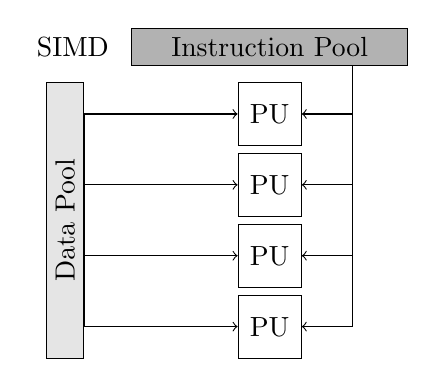
\begin{tikzpicture}
\draw (0.1,5.2) node {SIMD}; 
\node (rect) at (2.6,5.2) [draw,minimum width=3.5cm,fill=black!30] (ip) {Instruction Pool};
\node (rect) at (0,3) [rotate=90,draw,minimum width=3.5cm,fill=black!10] (dp) {Data Pool};
\node (rect) at (2.6,4.35) [draw,minimum width=.8cm,minimum height=.8cm] (pu1) {PU};
\node (rect) at (2.6,3.45) [draw,minimum width=.8cm,minimum height=.8cm] (pu2) {PU};
\node (rect) at (2.6,2.55) [draw,minimum width=.8cm,minimum height=.8cm] (pu3) {PU};
\node (rect) at (2.6,1.65) [draw,minimum width=.8cm,minimum height=.8cm] (pu4) {PU};
%\draw [->] ([yshift=2.35cm]dp) -- (pu1);
\draw[->] (dp.south) |- (pu1.west);
\draw[->] (dp.south) |- (pu2.west);
\draw[->] (dp.south) |- (pu3.west);
\draw[->] (dp.south) |- (pu4.west);

\draw[->] ([xshift=30pt]ip.south) |- (pu4.east);
\draw[->] ([xshift=30pt]ip.south) |- (pu3.east);
\draw[->] ([xshift=30pt]ip.south) |- (pu2.east);
\draw[->] ([xshift=30pt]ip.south) |- (pu1.east);
%\draw[arrow] (Small2B.north)--(Small2B|-Big2.south);s
%\draw [->] (dp) -- (pu1);
\end{tikzpicture}
}
\caption{Flynn taxonomy schematic representation of execution models}
\label{fig:1_HPC:flynn_taxonomy}
\end{figure}

In this classification~\cite{flynn1972some} from 1972, Michael J. Flynn presents the SISD, MISD, MIMD, and SIMD models represented on in table~\ref{tab:1_HPC:taxonomy_flynn} and figure~\ref{fig:1_HPC:flynn_taxonomy}.
Every of those execution model correspond to a specific machine and function.

\subsection{Single Instruction, Single Data: SISD}
This is the model corresponding to a single core CPU like in the Von Neumann model. 
This sequential model takes one instruction, operates on one data and the result is then store and the process continues over. 
SISD is important to consider as a reference computational time and will be taken in account in the next part for Amdahl's and Gustafson's laws.

\subsection{Multiple Instructions, Single Data: MISD}
This model can correspond to a pipelined computer.
Different operations are applied to the datum, which is transfered to the next computational unit and so on. 
This is the least common execution model.


\subsection{Multiple Instructions, Multiple Data: MIMD}
In MIMD every element executes its own instructions on its own data set. 
This can represent the behavior of a processor using several cores, threads or even the different nodes of a supercomputer cluster. 
Two subcategories are identified in this model:

\subsubsection{SPMD}
The Single Program Multiple Data model, SPMD, is the most famous parallelism way for HPC purpose: each process execute the same program. 
At opposite to SIMD the programs are the same but does not share the same instruction counter. 
This model was proposed for the first time in \cite{darema1988single} in 1988 using Fortran.
This is the common approach working with runtime like MPI. 
The programs are the same and the execution similar but based on their ID the processes will target different data. 

\subsubsection{MPMD}
The Multiple Program Multiple Data model is also know for HPC. 
Generally with a separation between a main program generating data for sub-programs. 
This is the model on which we work in part II regarding the Langford problem resolution using split of the resolution tree.

\subsection{Single Instruction, Multiple Data: SIMD}
This execution model corresponds to a many-core architecture like a GPU. 
SIMD can be extended from 2 to 16 elements for classical CPUs to hundreds and even thousands of core for GPGPUs. 
In the same clock, the same operation is executed on every process on different data. 
The best example stay the work on matrices like a stencil, same instruction executed on every element of the matrix. 

\subsection{SIMT}
\index{Single Instruction Multiple Threads}
We find another characterization to describe the new GPUs architecture: Single Instruction, Multiple Threads. 
This appears in one of NVIDIA's company paper~\cite{lindholm2008nvidia}. 
This model describes a combination of MIMD and SIMD architectures, every block of threads is working with the same control processor on different data and every block has its own instruction counter.  
This is the model we describe in part \ref{sec:CUDA} used for the \textit{warps} model in NVIDIA CUDA.

\section{Memory}
\label{sec:NORMA}
In addition of the execution model and parallelism the memory access patterns have a main role on performances especially in SIMD and MIMD. 
In this classification we identify three categories: UMA, NUMA and NoRMA for shared and distributed cases. 
This model have been pointed out in the Johnson's taxonomy\cite{johnson1988completing}.

%We can also find Error-Correcting Code, ECC, memory which implements a bunch of data correction algorithm to guaranty the validity of them when error is not allowed. 

%\todo{MCDRAM}
%\todo{3D memory}

\begin{figure}
\centering 
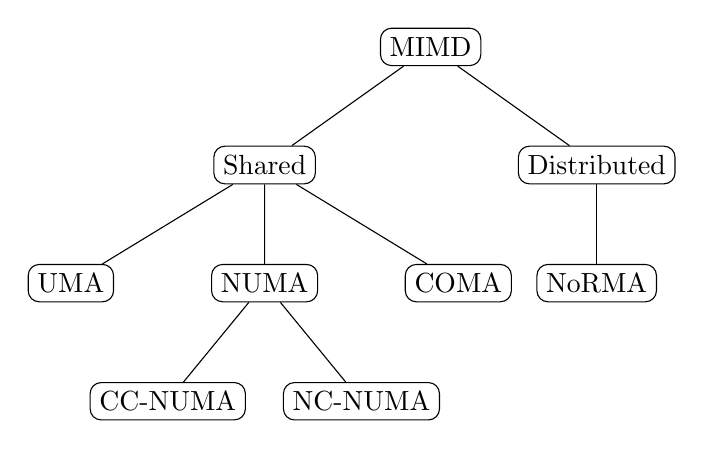
\begin{tikzpicture}[
   every node/.style = {
   level distance=1em,
   shape=rectangle, 
   rounded corners,
   draw, 
   align=center,
    top color=white%, 
   % bottom color=blue!20
   }]]
   \node {MIMD} [sibling distance=12em]
   child { node {Shared} [sibling distance=7em]
   child{node {UMA}} 
   child{node {NUMA}
   child{node {CC-NUMA}}
   child{node {NC-NUMA}}
   }
   child{node {COMA}}
   }
   child { node {Distributed}
   child { node {NoRMA}}
   };
\end{tikzpicture}
\caption{MIMD memory models}
\label{fig:1_HPC:mimd_memory_model}
\end{figure}

Those different types of memory for SIMD/MIMD model are summed up in figure~\ref{fig:1_HPC:mimd_memory_model}.

\subsection{Shared memory}
%In case of the SISD the memory access is just serial and no really rules needs to be set for its usage. 
When it comes to multi-threaded and multi-cores like MIMD or SIMD execution models, several kind of memory models are possible. 
We give a description of the most common shared memories architectures. 

\hspace*{-2cm}
\begin{figure}
\centering 
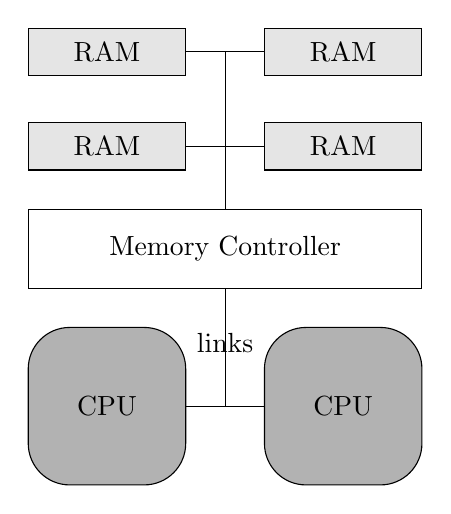
\begin{tikzpicture}
   \draw [rounded corners=15pt,fill=black!30] (0,0) rectangle (2,2) node[pos=.5] {CPU};
   \draw [rounded corners=15pt,fill=black!30] (3,0) rectangle (5,2) node[pos=.5] {CPU};

   \draw (0,2.5) rectangle (5,3.5) node[pos=.5] {Memory Controller};

   \draw (0,4) [fill=black!10] rectangle (2,4.6) node[pos=.5] {RAM};
   \draw (0,5.2) [fill=black!10] rectangle (2,5.8) node[pos=.5] {RAM};

   \draw (3,4) [fill=black!10] rectangle (5,4.6) node[pos=.5] {RAM};
   \draw (3,5.2) [fill=black!10] rectangle (5,5.8) node[pos=.5] {RAM};

   \draw [-] (2,1) -- (3,1);
   \draw [-] (2.5,1) -- (2.5,2.5);
	%\node at (2.5,2.2) {SDR, DDR, QDR};
	\node at (2.5,1.8) {links};

	\draw [-] (2.5,3.5) -- (2.5,5.5);
	\draw [-] (2,4.3) -- (3,4.3);
	\draw [-] (2,5.5) -- (3,5.5);
\end{tikzpicture}
\hspace{2cm}
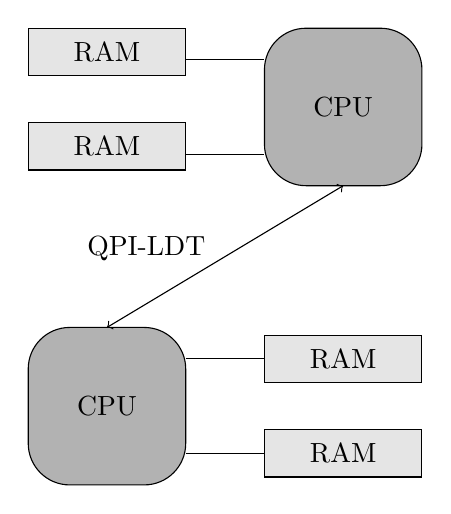
\begin{tikzpicture}
	\draw [rounded corners=15pt,fill=black!30] (0,0) rectangle (2,2) node[pos=.5] {CPU};
	\draw (3,0.1) [fill=black!10] rectangle (5,0.7) node[pos=.5] {RAM};
	\draw (3,1.3) [fill=black!10] rectangle (5,1.9) node[pos=.5] {RAM};
	\draw [-] (2,0.4) -- (3,0.4);
	\draw [-] (2,1.6) -- (3,1.6);

	\draw [rounded corners=15pt,fill=black!30] (3,3.8) rectangle (5,5.8) node[pos=.5] {CPU};
	\draw (0,4) [fill=black!10] rectangle (2,4.6) node[pos=.5] {RAM};
	\draw (0,5.2) [fill=black!10] rectangle (2,5.8) node[pos=.5] {RAM};
	\draw [-] (2,4.2) -- (3,4.2);
	\draw [-] (2,5.4) -- (3,5.4);

	\draw [<->] (1,2) -- (4,3.8);
	\node at (1.5,3) {QPI-LDT};
\end{tikzpicture}
%\hspace{1cm}
%\begin{tikzpicture}
%	\draw [rounded corners=15pt] (1,0) rectangle (3,2) node[pos=.5] {CPU};
%	\draw [rounded corners=15pt] (1,3.8) rectangle (3,5.8) node[pos=.5] {CPU};
%
%	\draw (0,2.1) rectangle (2,2.8) node[pos=.5] {RAM};
%	\draw (0,3.2) rectangle (2,3.8) node[pos=.5] {RAM};
%	
%	\draw (3,2.2) rectangle (5,2.8) node[pos=.5] {RAM};
%	\draw (3,2.2) rectangle (5,3.8) node[pos=.5] {RAM};
%
%\end{tikzpicture}
\caption{UMA vs NUMA memory models}
\label{fig:1_HPC:UMA_NUMA}
\end{figure}

\subsubsection{UMA}
\index{Unified Memory Access}
The Uniform Memory Access is a global memory shared by every threads or cores. 
In UMA every processor uses its own cache as local private memory. 
The addresses can be accessed directly by each processor which makes the access time ideal. 
The downside is that more processors require more buses and thus UMA is hardly scalable. 
The cache consistency problem also appears in this context and will be discussed in next part. 
Indeed, if a data is loaded in one processor cache and modified, this information need to be spread to the memory and maybe other processes cache. 

With the arising of accelerators like GPUs and their own memory, some constructors found ways to create UMA with heterogeneous memory. 
AMD creates the heterogeneous UMA, hUMA~\cite{rogers2013amd}, in 2013 allowing CPU and GPU to target the same memory area.

\subsubsection{NUMA}
\index{Non Unified Memory Access}
In Non Unified Memory Access every processor have access to its own private memory but allows other processors to access those area though Lightning Data Transport, LDT or Quick Path Interconnect, QPI, for Intel architectures. 

As we mention for the UMA memory, even if the processors does not directly access to the memory cache coherency is important. 
Two methods are possible: on one hand, the most used is Cache-Coherent NUMA (CC-NUMA) were protocols are used to keep data coherency through the memory. On the other hand No Cache NUMA (NC-NUMA) forces the processes to avoid cache utilization and write results in main memory losing all the benefits of caching data. 

\subsubsection{COMA}
\index{Cache-Only Memory Access}
In Cache-Only Memory Accesses, the whole memory is see as a cache from every processes.
Attraction memory is setting up and will attract the data near the process that will use those data. 
This model is less commonly use and lead to, in best cases, same results as NUMA.

\subsection{Distributed memory}
\index{No Remote Memory Access}
The previous models are based on shared memory, in the case where the processes can access memory of their neighbors processes. 
In some cases, like supercomputers, it would be too heavy for processors to handle the requests of all the others through the network. 
Each process or node will then possess its own local memory, that can be share with local processes. 
Then, in order to access to other nodes memory, communications through the network have to be done and copied in local memory. 
This distributed memory is called No Remote Memory Access (NoRMA).

\section{Performances characterization in HPC}
In the previous parts we described the different executions models, characterizations and memory models for HPC. 
Based on those tools we need to be able to emphasis the performances of a computer and a cluster. 

The performance can be of several kind. 
It can first be define by the speed of the processor itself with the frequency defined in GHz. 
This information is not perfect because the ALU is not busy all the time due to memory accesses, communications or side effects. 
It can be used to estimate the highest computational power of a machine. 
We define the notion of \textit{cycle} to be the number that determine the speed of a processor. 
This is the amount of time between two pulses of the oscillator. 
Higher cycles per seconds is better. 

\subsection{FLOPS}

\index{Floating-point Operations Per Second}
The Floating point Operations Per Second considers the number of floating-point operation that the system will executes in a second. 
They are an unit of performance for computers. 
Higher FLOPS is better. 
This is also the scale used to consider supercomputers computational power. 
For a cluster we can compute the theoretical FLOPS (peak) based on the processor frequency in GHz with:
\begin{equation}
FLOPS_{cluster} = \#nodes \times \frac{\#sockets}{\#node} \times \frac{\#cores}{\#socket} \times \frac{\#GHz}{\#core} \times \frac{FLOPS}{cycle}
\end{equation}
With $\#nodes$ the number of computational node of the system, $\frac{\#sockets}{\#node}$ the number of sockets ( = processor) per node, $\frac{\#cores}{\#socket}$ the number of core in the processor, $\frac{\#GHz}{\#core}$ the frequency of each core and finally $\frac{\#FLOP}{\#cycle}$ the number of floating-point operations per cycles for this architecture. 


On figure~\ref{tab:1_HPC:flops_year}, the scale of FLOPS and the year of the first world machine is presented.
The next milestone, the exascale, is expected to be reach near 2020.  

\begin{table}
\[\arraycolsep=1.4pt\def\arraystretch{2.2}
\begin{tabular}{| l | l | l || l | l | l |}
\hline
	%\rowstyle{\bfseries}
	\textbf{Name} & \textbf{FLOPS} & \textbf{Year} & \textbf{Name} & \textbf{FLOPS} & \textbf{Year} \\
	\hline
	\hline
	kiloFLOPS & $10^{3}$ & & petaFLOPS  & $10^{15}$ & 2005 \\ 
	\hline
	megaFLOPS & $10^{6}$ & & exaFLOPS   & $10^{18}$ & 2020 ? \\
	\hline
	gigaFLOPS & $10^{9}$ & $\approx$ 1980  & zettaFLOPS & $10^{21}$ & \\
	\hline
	teraFLOPS & $10^{12}$ & 1996 & yottaFLOPS & $10^{24}$ & \\
	\hline
	\end{tabular}
	\]
	\caption{Floating-point Operation per Second and years of reach in HPC.}
	\label{tab:1_HPC:flops_year}
\end{table}

FLOPS is the main way to represent a computer's performance but other ways exists like Instructions Per Seconds (IPS), Instructions per Cycle (IPC) or Operations Per Second (OPS).
Some benchmarks also provide their own metrics. 

\subsection{Power consumption}
Another way to consider machine performance is to estimate the number of operations regarding the power consumption. 
It can consider all the previous metrics like FLOPS, IPS, IPC or OPS. 
Benchmarks, like the Green500, consider the FLOPS delivered over the watts consumed. 
For nowadays architectures the many-cores architectures like GPUs seems to deliver the best FLOPS per watt ratio.

\subsection{Scalability}
The scalability express the way a program react to parallelism. 
When an algorithm is implemented on a serial machine and is ideal to solve a problem, one may consider to use it on more than one core, socket, node or even cluster. 
Indeed, one may expect less computation time, bigger problem or a combination of both while using more resources. 
This completely depend on the algorithm parallelization and is expressed through scalability. 
A scalable program will scale on as many processors as we give, whereas a poorly scalable one will give same of even worst results as the serial code.  
Scalability can be approach using speedup and efficiency.

\subsection{Speedup and efficiency}
The latency is the time required to complete a task in a program.
\index{Latency} 
Lower latency is better. 

The speedup compare the latency of both sequential and parallel algorithm. 
In order to get relevant results, one may consider the best serial program against the best parallel implementation.

Considering $n$, the number of processes, and $n=1$ the sequential case with $T_n$ the execution time working on $n$ processes and $T_1$ working on one process, the sequential execution time. 
The speedup can be defined using the latency by the formula: 
\index{Speedup}
\begin{equation}
\text{speedup} = S_n =  \frac{T_1}{T_n}
\end{equation}

\begin{figure}
\centering 
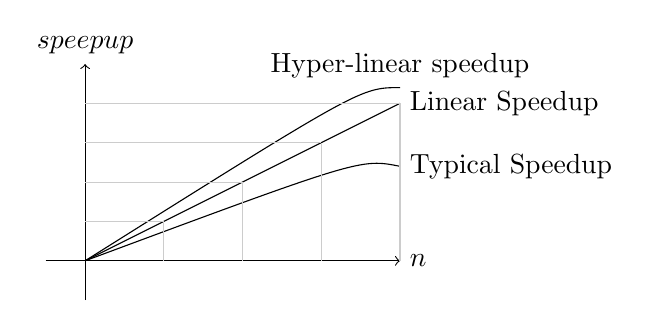
\begin{tikzpicture}
	\draw[->] (-.5,0) -- (4,0) node[right] {$n$};
	\draw[->] (0,-.5) -- (0,2.5) node[above] {$speepup$};
	\draw (0,0) -- (4,2) node[right] {\text{Linear Speedup}};
	\draw (0,0) .. controls (3.5,1.3) .. (4.,1.2) node[right] {\text{Typical Speedup}} ;
	\draw (0,0) .. controls (3.5,2.2) .. (4.,2.2) node[above] {\text{Hyper-linear speedup}} ;
   \draw[black!20] (1,0) -- (1,.5);
   \draw[black!20] (2,0) -- (2,1);
   \draw[black!20] (3,0) -- (3,1.5);
   \draw[black!20] (4,0) -- (4,2);
   \draw[black!20] (0,.5) -- (1,.5);
   \draw[black!20] (0,1) -- (2,1);
   \draw[black!20] (0,1.5) -- (3,1.5);
   \draw[black!20] (0,2) -- (4,2);
\end{tikzpicture}
\caption{Observed speedup: linear, typical and hyper-linear speedups}
\label{fig:1_HPC:speedup_obs}
\end{figure}

As shown on figure \ref{fig:1_HPC:speedup_obs} several kind of speedup can be observed. 
\paragraph{Linear: reference}
The linear speedup usually represents the target for every program in HPC. 
Indeed, having the speedup growing linearly as the number of processors grows is the ideal case. 
Codes fall typical into two cases, typical and hyper-linear speedup. 
\paragraph{Typical speedup}
This represents the most common observed speedup. 
As the number of processors grows, the program face several of the HPC walls like communications wall or memory wall. 
The increasing number of computational power is reduced to the sequential part or lose time in communications/exchanges. 
\paragraph{Hyper-linear speedup}
In some cases we can observe an hyper-linear speedup, meaning that the results in parallel are even better than the ideal case. 
This can occur if the program can fit exactly in memory for less data on each processor or even fit perfectly for the cache utilization. 
The parallel algorithm can also be way more efficient than the sequential one.\\

In addition to speedup, the efficiency is defined by the speedup divided by the number of workers: 
\index{Efficiency}
\begin{equation}
\text{efficiency} = E_n = \frac{S_n}{n} = \frac{T_1}{nT_n}
\end{equation}
The efficiency, usually expressed in percent, represents the evolution of the code stability to growing number of processors. 
As the number of processes grows, a scalable application will keep an efficiency near 100\%.

\subsection{Amdahl's and Gustafson's law}
The Amdahl's and Gustafson's laws are ways to evaluate the maximal possible speedup for an application taking in account different characteristics. 

\subsubsection{Amdahl's law}
\index{Amdahl's law}
The Amdahl's law\cite{amdahl1967validity} is used to find the theoretical speedup in latency of a program.
We can separate a program into two parts, the one that can be execute in parallel and the one that is sequential. 
The law states that even if we reduce the parallel part using an infinity of processes the sequential part will reach 100\% of the total computation time. 

Extracted from the Amdahl paper the law can be written as: 

\begin{equation}
S_n = \frac{1}{Seq + \frac{Par}{n}}
\end{equation}

Where $Seq + Par = 1$ and $Seq$ and $Par$ respectively the sequential and parallel ratio of a program.
Here if we use up to $n=\inf$ processes, $S_n \leq \frac{1}{Seq}$ the sequential part of the code become the most time consuming. 

And the efficiency become:
\begin{equation}
E_n = \frac{1}{n\times Seq + Par}
\end{equation}

\begin{figure}
\includegraphics[width=\textwidth]{\locpath/figures/chap1/speedup_laws.png}
\caption{Theoretical speedup for Amdahl's (left) and Gustafson's (right) law}
\label{fig:1_HPC:speedup_laws}
\end{figure}

A representation of Amdahl's speedup is presented on Fig.~\ref{fig:1_HPC:speedup_laws} with varying percentage of serial part. 
The parallel part is like $Par = (100-Ser)\%$.

\subsubsection{Gustafson's law}
\index{Gustafson's law}
The Amdahl's law is focused on time with problem of the same size. 
John L. Gustafson's idea is that using more computational units, the problem size can grow accordingly. 
He considered a constant computation time with evolving problem, growing the size accordingly to the number of processes. 
Indeed the parallel part grows as the problem size do, reducing the percentage of the serial part for the overall resolution.

The speedup can now be estimated by:
\begin{equation}
S_n = Seq + Par \times n
\end{equation}

And the efficiency: 
\begin{equation}
E_n = \frac{Seq}{n} + Par
\end{equation}


Both Amdahl's and Gustafson's law are applicable and they represent two solution to check the speedup of our applications. 
The strong scaling\index{Strong scaling}, looking at how the computation time vary evolving only the number of processes, not the problem size. 
The weak scaling\index{Weak scaling}, at opposite to strong scaling we look how the computation time evolute varying the problem size keeping the same amount of work per processes. 

\section{Conclusions}

In this chapter we presented the different basic tools to be able to understand HPC: the Von Neumann model that is implemented in every nowadays architecture; the Flynn taxonomy that is in constant evolution with new paradigms like recent SIMT from NVIDIA. 
We also presented the memory types that will be use at different layers in our clusters, from node memory, CPU-GPGPU shared memory space to global fast shared memory. 
We finished by presenting the most important laws with Amdahl's and Gustafson's laws.
We introduced the concept of strong and weak scaling that will lead our tests through all the examples in Part II and Part III.

Those models have now to be confronted to the reality with hardware implementation and market reality, the vendors. 
The next part will introduce chronologically hardware and their optimization but always keeping a link with the models presented in this part. 
As there is always a gap between models and implementation we will have to find way to rank and characterize those architecture. 
This will be discuss in the last chapter. 



%%%%%%%%%%%%%%%%%%%%%%%%%%%%%%%%%%%%%%%%%%%%%%%%%%%%%%%%%%%%%%%%%%%%%
%																	%
%	CHAPTER TWO, HARDWARE IN HPV									%
%																	%
%%%%%%%%%%%%%%%%%%%%%%%%%%%%%%%%%%%%%%%%%%%%%%%%%%%%%%%%%%%%%%%%%%%%%

%%%%%%%%%%%%%%%%%%%%%%%%%%%%%%%%%%%%%%%%%%%%%%%%%%%%%%%%%%%%%%%%%%%%%
%																	%
%	CHAPTER TWO, HARDWARE IN HPV									%
%																	%
%%%%%%%%%%%%%%%%%%%%%%%%%%%%%%%%%%%%%%%%%%%%%%%%%%%%%%%%%%%%%%%%%%%%%

\chapter{Hardware in HPC}

\section{Introduction}

Optimization can't be done without a good knowledge of the architecture of device, machine, or computer. 
Indeed, nowadays software and API try to take care of most of the optimizations but the last percents of gain always need to be architecture dependent. 
In this chapter we describe the most important devices architecures from classical processors, General Purpose Graphics Processing Units (GPGPUs), Field Programmable Gate Arrays (FPGAs) and Application-specific integrated circuits (ASICs).
Then those independants elements are use together in order to build supercomputers. 
The way they are arranged and the nodes interconnection is something that matters at large scale. 

\section{Architectures}
In this section we will describe the main nowadays architecture from HPC world and their specificities.

The CPU, as we know it today, begins its history with \textit{Texas Instruments Inc} and the first patent describing a CPU is "Computing systems cpu" proposed by \textit{Gary Boone} and published in 1973.
It is the reflection of the Von Neumann Machine we presented in Chapter I. 

From this first version plenty of optimizations arised. 
\begin{description}[noitemsep,nolistsep]
	\item[Multiple CPU cores] Multiple CPU cores on the same die. They can have independant or share part of the cache and access to the same main memory. The first machine were the IBM power4 with dual core.
	\item[In/Out-Of-Order] In-order-process is the one describes in previous chapter, the CU fetches instruction in memory, then the operands and the ALU computes, and finally the results is stored in memory. 
	In this model the time to perform an instruction, cumulation of instruction fetching + operand fetching + computation + store the resul, can be high and the ALU itself is busy only one step for computation itself. The idea of Out-of-order is to compute the instructions without following the PC order. Indeed, for independant tasks (this is know based on dependancy graphs) while the process fetch the next instructions data, the ALU can perform another operation with already available data. 
	\item[Prefetching] When a data is not available in L1 cache, it has to be moved from either L2 to L1 or L3 to L2 to L1 or in the worst case RAM to L3 to L2 to L1. Prefecthing technology is a way to, knowing the next instructions operands, prefetch the data in closer cache. The prefetch can either be hardware or software implemented and can concern data and even instructions.
	\item[Vectorization] Processors allows the instructions to be executed at the same time in a SIMD manner. If the same instruction is executed on coalescent data they can be executed in the same clock cycle. 
	Of course this tool require specific care during coding. 
\end{description}
Those optimizations can be found either in the classical processor model or accelerators.  

\subsection{Classical processors}

Nowadays processors share mostly the same architecture. 
They are called multi-cores and provide up to 2 to 16 cores and each constructor have its own specificities. 
Those processors are called "Host" because they are usually bootable and most of the accelerators need to be attached to them in order to work.

\subsubsection{Intel}

Intel was created in 1968 by a chemist and a physicists, Gordon E. Moore and Robert Noyce, in Montain View, California. 
Nowadays processors are mostly Intel ones, this world leader equips around 90\% of the supercomputers (November 2017 TOP500 list).
Since 2007 Intel adopted a production model called the "Tick Tock", presented on Fig.~\ref{fig:1_HPC:intel_tick_tock}.

\begin{figure}
\begin{center}
\includegraphics[width=.8\textwidth]{\locpath/figures/chap1/intel_tick_tock.png}
\caption{Intel Tick-Tock model}
\label{fig:1_HPC:intel_tick_tock}
\end{center}
\end{figure}

Since its creation the model followed the same fashion, a new manufacturing technology like shrink of the chip with better engraving on a "Tick" and a new microarchitecture delivered on a "Tock".
The Intel processors for HPC are called Xeon and features ECC memory, higher number of cores, large RAM support, large cache-memory, Hyperthreading, etc. compared to desktop processors. 
Every new processor have a code name. 
The last generations are chronologically called Westemere, Sandy Bridge, Ivy Bridge, Haswell, Broadwell, Skylake and Kaby lake. 
Kaby Lake, the last architecture of processor, does not exactly fit the usual "Tick-Tock" process because it is just based on optimizations of the Skylake architecture. 
It is produce like Skylake in 14nm.
This model seems to be hard to maintain due to the difficulties to engrave in less than 10nm with quantum tunneling. 

\subsubsection{Hyperthreading}
Another specificity of Intel processor is Hyperthreading (HT). 
This technology makes a single physical processor appearing as two logical processors for user's level.
In fact a processors embedding 8 cores will appear as a 16 cores for user. 
Adding more computation per node can technically allows the cores to switch context when data are fetched from the memory using the processor 100\% during all the computation. 
A lot of studies have been released on HT from Intel itself~\cite{marr2002hyperthreading} to other studies~\cite{bononi2006exploring,leng2002empirical}.
This does not fit to all the cases and can be disable for normal use of the processors. 

\subsubsection{Xeon Phi}
Another specific HPC product from Intel is the Xeon Phi. 
This device can be considered as a Host or Device/Accelerator machine. 
Intel describes it as "a bootable host processor that delivers massive parallism and vectorization".
This architecture embedded multiple multi-cores processors interconnected. 
This is call Intel's Many Integrated Core (MIC).
The architectures names are Knights Ferry, Knights Ferry, Knights Corner and Knight Landing~\cite{sodani2016knights}. 
The last architecture, Knight Hill, was recently canceled by Intel. 
The main advantage of this architecture compared to GPGPUs is the x86 compatibility of the embedded cores and the fact this device can boot and use to drive other accelerators. 
They also feature more complex operations and handle double precision natively. 

\subsubsection{ARM}
Back in 1980s, ARM stood for Acorn RISC Machine in reference of the first company implementing this kind of architecture, Acorn Computers. 
This company later changed to Advanced RISC Machine (ARM). 
ARM is a specific kind of CPU based on RISC architecture as its ISA depsite usual processors using CISC.
The downside of CISC machines makes them hard to create and they require way more energy to work. 
The ISA from the RISC is simplier and requires less transistors to operate. 
Therefore, the energy required and the heat dissipated is less important. 
It would then be easier to create massively parallel processors based on ARM. 
On the other hand, simple ISA impose more work on the source compilation to fit the simple architecture. 
That makes the instructions sources longer and therefore more single instructions to execute. 

The ARM company provide several version of ARM processors named Cortex-A7X, Cortex-A5X and Cortorx-A3X respectively balancing highest-performances, performances and efficiency and less power consumption. 
We find here the same kind of naming as Intel processors. 

The new ARMv8 architecture starts to have the tools to target HPC context~\cite{rico2017arm}.
The european approach towards energy efficient HPC, Mont-Blanc project\footnote{http://montblanc-project.eu/}, already constructs ARM based supercomputers. 
For the Exascale project in Horizon 2020 this project focus on using ARM-based systems for HPC with many famous contributors with Atos/Bull as a project coordinator, ARM, French Alternative Energies and Atomic Energy Commission (CEA), Barcelona Supercomputing Center (BSC), etc.
The project is decomposed in several steps to finaly reach Exascale near 2020. 
The third step, Mont-Blanc 3, is about to work on a pre-exascale prototype powered by Cavium’s ThunderX2 ARM chip based on 64-bits ARMv8.

\subsection{GPGPU}

GPUs are based on the SIMD model of the Flynn taxonomy presented previously, \emph{Single Instruction, Multiple Data}.
The specific execution model is called SIMT (\emph{Single Instruction, Multiple Thread}). It enables the execution of millions of coordinated threads in a data-parallel mode. 
Two main companies provide GPGPUs for HPC: NVIDIA and AMD.
We will present them in that order and conclude on the differences. 

\subsubsection{NVIDIA GPU architecture}

The NVIDIA company was fonded in April 1993 in Santa Clara, Carolina, by three persons in which Jensen Huang, the actual CEO.
Its name seems to come from \textit{invidia} the latin word for Envy and vision, for the graphics generation. 

Known as the pioner in graphics, cryptocurrency, portable devices and now AI, it seems to be even the creator of the name "GPU".
It GPU, inspired from visualisation and gaming at a first glance, is available as a dedicated device  since the Tesla. 
The public GPUs can also be use for dedicated computation but does not feature ECC memory, double precision or special functions/FFT cores. 

\begin{figure*}[t!]
\centering
\setlength\fboxsep{0pt}
\setlength\fboxrule{0.25pt}
\includegraphics[scale=0.6]{\locpath/figures/chap1/smx}
\caption{NVIDIA GPU and CUDA architecture overview}
 \label{fig:chap1_gpu}
%\vspace{-0.8cm} 
\end{figure*}

As presented in Fig.\ref{fig:chap1_gpu}, NVIDIA GPUs include many \emph{Streaming Multiprocessors} (SM), each of which is composed of many \emph{Streaming Processors} (SP). In the Kepler architecture, the SM new generation is called SMX.
%
%In the CUDA programing model~\cite{cuda}, the GPU works as a SIMT co-processor of a conventional CPU. 
Grouped into \emph{blocks}, \textit{threads} execute \emph{kernel} functions synchronously.
Threads within a block can cooperate by sharing data on an SMX and synchronizing their execution to coordinate memory accesses; inside a block, the scheduler organizes \emph{warps} of 32 threads which execute the instructions simultaneously.
The blocks are distributed over the GPU SMXs to be executed independently.

\paragraph{Memory, bandwidth and streams:}

In order to use data in a CUDA kernel, it has to be first created on the CPU, allocated on the GPU and then transferred from the CPU to the GPU; after the kernel execution, the results have to be transferred back from the GPU to the CPU. 
GPUs consist of several memory categories, organized hierarchically and differing by size, bandwidth and latency.   
On the one hand, the device's main memory is relatively large but has a slow access time due to a huge latency. 
On the other hand, each SMX has a small amount of shared memory and L1 cache, accessible by its SPs, with faster access, and registers organized as an SP-local memory. 
SMXs also have a constant memory cache and a texture memory cache.
%, that are linked to the constant and texture memories physically located in the device memory: these are read-only and have faster access time than the rest of the memory categories.
Reaching optimal computing efficiency requires considerable effort while programming.
Most of the global memory latency can then be hidden by the threads scheduler if there is enough computational effort to be executed while waiting for the global memory access to complete. Another way to hide this latency is to use streams to overlap kernel computation and memory load. 

\paragraph{Threads synchronization:}
It is also important to note that branching instructions may break the threads synchronous execution inside a warp and thus affect the program efficiency. 
This is the reason why test-based applications, like combinatorial problems that are inherently irregular, are considered as bad candidates for GPU implementation. 
%This is particularly true with regard to combinatorial problems resolution. 
Thus we intend to provide a way to regularize their execution, in order to get good acceleration with GPU computation. 

\paragraph{HPC tools}
Specific tools have been made for HPC in the NVIDIA GPGPUs. 
\begin{description}[noitemsep,nolistsep]
	\item[Dynamic Parallelism] This feature allow the GPU kernels to run other kernels themself. This feature 
	\item[Hyper-Q] This technology enable several CPU threads to execute kernels on the same GPU simultaneously. This can help to reduce the synchronization time and idle time of CPU cores for specific applications.
	\item[NVIDIA GPU-Direct] GPUs' memory and CPU ones are different and the Host much push the data on GPU before allowing it to compute. GPU-Direct allows direct transferts from GPU devices through the network. Usually implemented using MPI.  
\end{description}

We give details on the GPU we mainly used in this study in the ROMEO supercomputer center. 

\paragraph{Details on K20X}
This NVIDIA Tesla Kepler GPU is based on the GK110 graphics processor describes in the whitepaper\cite{nvidia2012nvidias} on 28nm process.
This GPU comes in active and passive cooling with respectively K20Xc and K20Xm.
This GPU embedded 2688 CUDA cores distributed in 14 SMX (we note that GK110 normally provides 15 SMX but only 14 are present4 on the K20X).
In this model each SMX contains 192 single precisions cores, 64 double precision cores, 32 special function units and 32 load/store units.
In a SMX the memory provides 65536 32-bits registers, 64KB of shared memory L1 cache, 48KB of read-only cache
The L2 cache is 1546KB shared by the SMX for a total of 6GB of memory adding the DRAM.
The whole memory is protected using Single‐Error Correct Double‐Error Detect (SECDED) ECC code.
The power consumption is estimated to 225W.
This GPGPU is expected to produce 1.31 TFLOPS for double-precision and 3.95 TFLOPS of single-precision.

\subsubsection{AMD}
Another company is providing GPUs for HPC, Advanced Micro Devices (AMD). 
In front of the huge success of NVIDIA GPU that leads from far the HPC market, it is hard for AMD to place its GPGPUs. 
Their HPC GPUs are called FirePro.
They are targeting using a language near CUDA called OpenCL. 
An interessant creation of AMD are the Accelerated Processing Units (APUs) which embedded the processor and the GPU on the same die since 2011. 
This solution allows them to target the same memory. 

\subsection{FPGA and ASIC}
Field Programmable Gates Array are device that can de reprogram to fit the needs of the user after their construction.
The leader was historically Altera with the Stratix, Arria and Cyclone FPGAs and is now part of Intel. 
With the FPGAs the user have access to the hardware itself and can design its own circuit. 
Nowadays FPGA can be targeted with OpenCL programming language. 
The arrival of Intel in this market promess the best hopes for HPC version of FPGAs. 
The main gap for users is the circuit building itself, perfect to respond to specific needs but hard to setup. 

ASICs are dedicated device construct for on purpose. 
An example of ASIC can be the Gravity Pipe (GRAPE) which is dedicated to compute gravitation given mass/positions.
Google leads the way for ASIC and just created its dedicated devices to boost AI bots. 

\section{Interconnection and clusters}

\subsection{Interconnects}
Interconnect is the way the nodes of a cluster are connected together. 
Several topologies exists from point to point to multi dimensional torus.

\begin{table}
\begin{center}
\[\arraycolsep=0.pt\def\arraystretch{1.2}
\begin{tabular}{| l | l | l || l | l | l | }
\hline
\textbf{Type} & \textbf{SubType} & \textbf{Diameter} & \textbf{Name} & \textbf{Gbs} & \textbf{Year} \\
\hline
\hline
Trees & & & & & \\
& Fat Tree & & & & \\
& k-ary tree & & & & \\
& Extended Fat Tree & & & &\\
\hline
Mesh/Torus & & & & & \\
& k-ary n-mesh & & & & \\
& k-ary n-cube & & & & \\
\hline
Dragonfly & & & & & \\
\hline
HyperX & & & & &  \\
\hline
\end{tabular}
\]
\caption{InfiniBand technologies}
\label{fig:1_HPC:topology}
\end{center}
\end{table}

\todo{Finir table}
\todo{Ajouter schema des topologies ?}
The Fig.\ref{fig:1_HPC:topology} list the most famous interconnection network and their diameters.

InfiniBand (IB) is the most spread technology used for interconnect with different kind of bandwith presented in Fig.\ref{fig:1_HPC:infiniband}.

\begin{table}
\begin{center}
\[\arraycolsep=0.pt\def\arraystretch{1.2}
\begin{tabular}{| l | l | l || l | l | l | }
\hline
\textbf{Name} & \textbf{Gbs} & \textbf{Year} & \textbf{Name} & \textbf{Gbs} & \textbf{Year} \\
\hline
\hline
Single DR & 2.5 & 2003 & Enhanced DR & 25 & 2014 \\
\hline
Double DR & 5 & 2005 & Highg DR & 50 & 2017 \\
\hline
Quad DR & 10 & 2007 & Next DR & 100 & 2020 \\
\hline
Fourth DR & 14 & 2011 & & &  \\
\hline
\end{tabular}
\]
\caption{InfiniBand technologies}
\label{fig:1_HPC:infiniband}
\end{center}
\end{table}

\subsection{TOP500 remarkable supercomputer}
The TOP500 is the reference benchmarks for the world size supercomputers. 
Most of the TOP10 machines have specific architecture and, of course, the most efficient ones. 
In this section we give details on several supercomputers about their interconnect, processors and specific accelerators. 

\subsubsection{Sunway Taihulight}

Sunway Taihulight is the third Chinese supercomputer to be ranked in the first position of the TOP500 list. 
A recent report from Jack J. Dongarra, a figure in HPC, decrypt the architecture of this supercomputer\cite{dongarra2016report}. 
The most interessant point is the conception of this machine, completely done in China. 
The Sunway CPUs were invented and built in China, the Vendor is the Shanghai High Performance IC Design Center. 

\begin{figure}
\centering
\includegraphics[scale=1]{\locpath/figures/Chap1/report_sunway_CPE}
\caption{Sunway Taihulight node architecture from \textit{Report on the Sunway TaihuLight System}, Jack Dongarra, June 24, 2016.}
\label{fig:chap1_report_sunway_CPE}
\end{figure}

The SW26010, a many core architecture processor, features 260 cores based on RISC architecture and a specific conception depicted on Fig.\ref{fig:chap1_report_sunway_CPE}. 
The processor is composed of the master core, a Memory Controller (MC), a Management Processing Element (MPE) that manages the Computing Processing Elements (CPE) which are the slaves cores. 

The interconnect network is called Sunway Network and connected using Melloanix Host Channel Adapter (HCA) and switches. 
This is a five level interconnect going through computing nodes, computing board, supernodes and cabinets to the complete system.
The total memory is 1.31 PB and the number of cores available is 10,649,600.
The peak performance is 125.4 PFLOPS and the Linpack is 93 PFLOPS which induce 74.16\% of efficiency. 

\subsubsection{Piz Daint}
The supercomputer of the CSCS, Swiss National Supercomputing Center, is currently ranked 2nd of the November 2017 TOP500 list. 
This GPU accelerated GPU is a most powerful representative of the hybrid architecture featuring processor and accelerators. 

\subsubsection{K-Computer}
K-Computer was the top 1 supercomputer of TOP500 2011 list. 

The TOFU interconnect network makes the K-Computer unique~\cite{ajima2009tofu} and stands for TOrus FUsion.
This interconnect mixes a 6D Mesh/Torus interconnect.


\subsubsection{Sequoia/Mira}
Sequoia supercomputer was top 1 of the TOP500 2012 list. 
It is based on BlueGene from IBM.
The BlueGene project made up to three main architectures with BlueGene/L, BlueGene/P and BlueGene/Q.

\section{ROMEO Supercomputer}

The ROMEO supercomputer center is the computation center of the Champagne-Ardenne region in France. 
Hosted since 2002 by the University of Reims Champagne-Ardenne, this so called meso-center (French name for software and hardware architectures) is used for HPC for theoric research and domain science like applied mathematics, physics, biophysics and chemistry. 

This project is support by the Champagne-Ardenne region and the CEA (French Alternative Energies and Atomic Energy Commission), aim to host research and production codes of the region for industrial, research and academics purposes. 

We are currently working on the third version of ROMEO, installed in 2013. 
As many of our tests in this study have been done on this machine, we will carefully describe its architecture. 

This supercomputer was ranked 151st in the TOP500 and 5th in the GREEN500 list. 

\subsection{ROMEO hardware architecture}
ROMEO is a Bull/Atos supercomputer composed of 130 BullX R421 computing nodes. 

Each node is composed of two processors Intel Ivy Bridge 8 coeurs @ 2,6 GHz. 
Each processor have access to 16GB of memory for a total of 32GB per node, the total memory if 4.160TB. 
Each processor if linked, using PCIe-v3, to an NVIDIA Tesla K20Xm GPGPU. 
This cluster provide then 260 processors for a total of 2080 CPU cores and 260 GPGPU providing 698880 GPU cores. 
The computation nodes are interconnected with an Infiniband QDR non-blocking network structured as a FatTree. 
The Infiniband is a QDR providing 10GB/s. 

The storage for users is 57 TB and the cluster also provide 195 GB of Lustre and 88TB of parallel scratch filesystem. 

In addition to the 130 computations nodes, the cluster provides a visualization node NVIDIA GRID with two K2 cards and 250GB of DDR3 RAM. 
The old machine, renamed Clovis, is always available but does not features GPUs. 

The supercomputer supports MPI with GPU Aware and GPUDirect. 

\section{Conclusion}

In this chapter we reviewed the most important nowadays hardware architectures and technologies. 
In order to use the driver or API in the most efficient way we need to keep in mind the way the data and instructions are proceed by the machine. 

As efficiency is based on computation power but also communications we showed different interconnection topologies and their specificities. 

The TOP500 supercomputers presented here are a perfect use case of the tehcnologies presented and reflect the best human can do with nowadays systems.
They also show that every architecture is unique in its construction and justify the optimization work dedicated to reach performance.   

%%%%%%%%%%%%%%%%%%%%%%%%%%%%%%%%%%%%%%%%%%%%%%%%%%%%%%%%%%%%%%%%%%%%%
%																	%
%	CHAPTER THREE, SOFTWARE AND API									%
%																	%
%%%%%%%%%%%%%%%%%%%%%%%%%%%%%%%%%%%%%%%%%%%%%%%%%%%%%%%%%%%%%%%%%%%%%

%%%%%%%%%%%%%%%%%%%%%%%%%%%%%%%%%%%%%%%%%%%%%%%%%%%%%%%%%%%%%%%%%%%%%
%                                                                   %
%	CHAPTER THREE, SOFTWARE AND API                                   %
%                                                                   %
%%%%%%%%%%%%%%%%%%%%%%%%%%%%%%%%%%%%%%%%%%%%%%%%%%%%%%%%%%%%%%%%%%%%%

\chapter{Software in HPC}

\section{Introduction}
After presenting the rules of HPC and the hardware that compose the cluster, we introduce the most famous ways to target those architectures and supercomputers with programming models.
Then, fitting those models, we present the possible options in the language, the API, the distribution and the accelerators code. 

This chapter details the most important programming models and the software options for HPC programming and include the choices we made for our applications.
Then it presents the software used to benchmark the supercomputers. 
We present here the most famous, the TOP500, GRAPH500, HPGC and GREEN500 to give their advantages and weaknesses. 

\section{Parallel and distributed programming Models}
The Flynn taxonomy developed in chapter 1 was a characterization of the executions models. 
This model can be extended to programming models which are an extension of MIMD. 
We consider here a \textit{Random Access Machine} (RAM). 
The memory of this machine consists of an unbounded sequence of registers each of which may hold an integer value. 
In this model the applications can access to every memory words directly in write or read manner.
There is three main operations: load from memory to register; compute operation between data; store from register to memory. 
This model is use to estimate the complexity of sequential algorithms. 
If we consider the unit of time of each operation (like in cycle) we can have an idea of the overall time of the application.
We identify two types of RAM, the Parallel-RAM using shared memory and the Distributed-RAM using distributed memory. 

\subsection{Parallel Random Access Machine}
The Parallel Random Access Machine \cite{fortune1978parallelism}, PRAM, is a model in which the global memory is shared between the processes and each process have its own local memory/registers.
The execution is synchronous, processes execute the same instructions at the same time. 
In this model each process is identify with its own index enabling to target different data. 
The problem in this model will be the concurrency in reading (R) and writing (W) data as the memory is shared between the processes.
Indeed, mutual exclusion have to be set with exclusive (E) or concurrent (C) behaviors and we find 4 combinations: EREW, ERCW, CREW and CRCW.
As the reading is not critical for data concurrency the standard model will be Concurrent Reading and Exclusive Writing: CREW.

\subsection{Distributed Random Access Machine}
For machine that base their memory model on NoRMA the execution model can be qualify of Distributed Random Access Machine, DRAM.
It is based on NoRMA memories detailed in part \ref{sec:NORMA}.
This model is in opposition to PRAM because the synchronization between processes is made by communications and messages. 
Those communications can be of several kind and depend of physical architecture, interconnection network and software used.

\subsection{H-PRAM}
A DRAM can be composed of an ensemble of PRAM system interconnected. 
Each of them working on their own data and instructions. 
This is an intermediate model between PRAM and DRAM having a set of shared memory and synchronous execution, the overall execution being asynchronous and having distributed memory.

\begin{figure}
\begin{center}
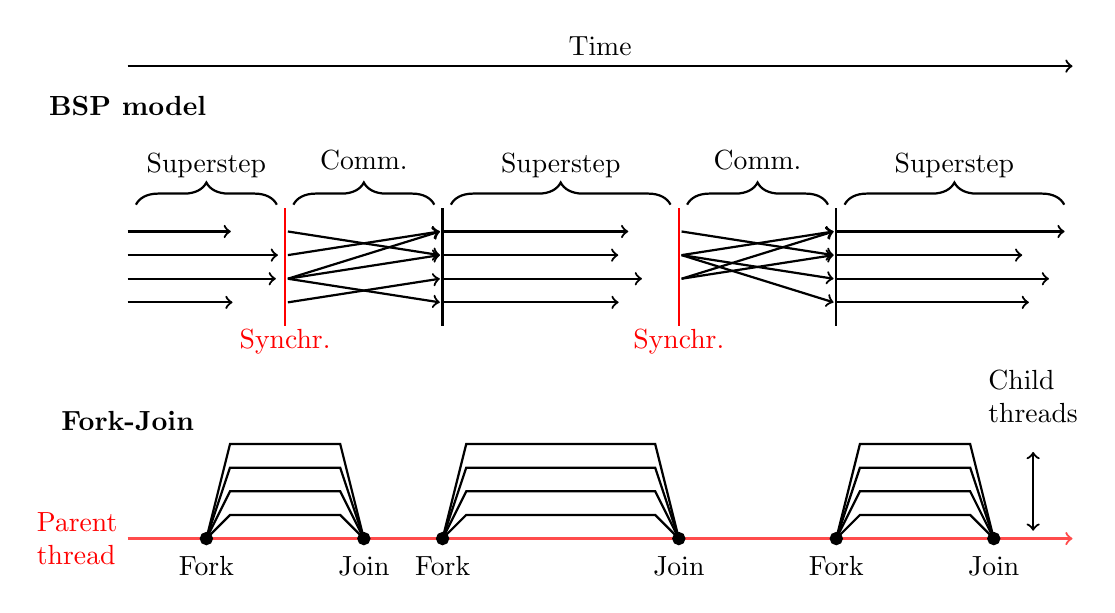
\begin{tikzpicture}[thick]
% Fork Join model
\coordinate (begin) at (0,0);
\coordinate (f0) at (1,0);
\coordinate (j0) at (3,0);

\coordinate (f1) at (4,0);
\coordinate (j1) at (7,0);

\coordinate (f2) at (9,0);
\coordinate (j2) at (11,0);

\coordinate (end) at (12,0);

\node at ([yshift=1.5cm]begin) {\textbf{Fork-Join}};


% Main threads and info
\draw[->,red!70] (0,0) -- (f0) -- (j0) -- (f1) -- (j1) -- (f2) -- (j2) -- (end);
\node[anchor=east,red,align=left] (0,0) {Parent\\thread};
\foreach \x in {0,...,2}{
\draw[fill,black,thick] (f\x) circle [radius=2pt] ;
\draw[fill,black,thick] (j\x) circle [radius=2pt] ;
\node at ([yshift=-10pt]f\x) {Fork}; 
\node at ([yshift=-10pt]j\x) {Join}; 
}

% Thread
\foreach \x in {1,...,4}{
  \draw[thick] (f0) -- ([yshift=\x*.3cm,xshift=.3cm]f0) -- ([xshift=-.3cm,yshift=\x*.3cm]j0) -- (j0);

  \draw[thick] (f1) -- ([yshift=\x*.3cm,xshift=.3cm]f1) -- ([xshift=-.3cm,yshift=\x*.3cm]j1) -- (j1);

  \draw[thick] (f2) -- ([yshift=\x*.3cm,xshift=.3cm]f2) -- ([xshift=-.3cm,yshift=\x*.3cm]j2) -- (j2);
}

% Name of threads
\draw[<->] (11.5,0.1) -- (11.5,1.1) node[anchor=south,yshift=7pt,align=left] {Child\\threads};


% BSP model
\coordinate (begin) at (0,3);

\coordinate (s0) at (2,3);
\coordinate (c0) at (4,3);
\coordinate (s1) at (7,3);
\coordinate (c1) at (9,3);
%\coordinate (s2) at (9,3);

\coordinate (end) at (12,3);

% Figure name 
\node at ([yshift=2.5cm]begin) {\textbf{BSP model}};

\draw [decorate,decoration={brace,amplitude=8pt,raise=4pt},yshift=0pt] ([yshift=1.1cm,xshift=3pt]begin) -- ([yshift=1.1cm,,xshift=-3pt]s0) node [black,midway,above,yshift=10pt] {Superstep};

\draw [decorate,decoration={brace,amplitude=8pt,raise=4pt},yshift=0pt] ([yshift=1.1cm,xshift=3pt]s0) -- ([yshift=1.1cm,,xshift=-3pt]c0) node [black,midway,above,yshift=13pt] {Comm.};

\draw [decorate,decoration={brace,amplitude=8pt,raise=4pt},yshift=0pt] ([yshift=1.1cm,xshift=3pt]c0) -- ([yshift=1.1cm,,xshift=-3pt]s1) node [black,midway,above,yshift=10pt] {Superstep};

\draw [decorate,decoration={brace,amplitude=8pt,raise=4pt},yshift=0pt] ([yshift=1.1cm,xshift=3pt]s1) -- ([yshift=1.1cm,,xshift=-3pt]c1) node [black,midway,above,yshift=13pt] {Comm.};

\draw [decorate,decoration={brace,amplitude=8pt,raise=4pt},yshift=0pt] ([yshift=1.1cm,xshift=3pt]c1) -- ([yshift=1.1cm,,xshift=-3pt]end) node [black,midway,above,yshift=10pt] {Superstep};


% Draw vertical lines 
\foreach \x in {0,...,1}{
\draw[red] ([yshift=-.3cm]s\x) -- ([yshift=1.2cm]s\x);
\node[red] at ([yshift=-.5cm]s\x) {Synchr.};

\draw ([yshift=-.3cm]c\x) -- ([yshift=1.2cm]c\x);
%\node at ([yshift=-.5cm]s\x) {Synchr.};
}

\foreach \x in {0,...,3}{
  \draw[->] ([yshift=\x*.3cm]begin) -- ([yshift=\x*.3cm,xshift=((rnd)*-20pt-2pt)]s0);
  \draw[->] ([yshift=\x*.3cm]c0) -- ([yshift=\x*.3cm,xshift=((rnd)*-20pt)-2pt]s1);
  \draw[->] ([yshift=\x*.3cm]c1) -- ([yshift=\x*.3cm,xshift=((rnd)*-20pt)-2pt]end);
  %\draw[->] ([yshift=\x*.3cm]s2) -- ([yshift=\x*.3cm,xshift=((rnd)*-20pt)-2pt]end);
}

% Add comms 
% comm 0 
\draw[->] ([xshift=1pt,yshift=.3cm]s0) -- ([xshift=-1pt,yshift=.9cm]c0);
\draw[->] ([xshift=1pt,yshift=0]s0) -- ([xshift=-1pt,yshift=.3cm]c0);
\draw[->] ([xshift=1pt,yshift=.3cm]s0) -- ([xshift=-1pt,yshift=0]c0);
\draw[->] ([xshift=1pt,yshift=.6cm]s0) -- ([xshift=-1pt,yshift=.9cm]c0);
\draw[->] ([xshift=1pt,yshift=.3cm]s0) -- ([xshift=-1pt,yshift=.6cm]c0);
\draw[->] ([xshift=1pt,yshift=.9cm]s0) -- ([xshift=-1pt,yshift=.6cm]c0);

% comm 1
\draw[->] ([xshift=1pt,yshift=.6cm]s1) -- ([xshift=-1pt,yshift=.9cm]c1);
\draw[->] ([xshift=1pt,yshift=.6cm]s1) -- ([xshift=-1pt,yshift=.3cm]c1);
\draw[->] ([xshift=1pt,yshift=.6cm]s1) -- ([xshift=-1pt,yshift=0]c1);
\draw[->] ([xshift=1pt,yshift=.3cm]s1) -- ([xshift=-1pt,yshift=.9cm]c1);
\draw[->] ([xshift=1pt,yshift=.3cm]s1) -- ([xshift=-1pt,yshift=.6cm]c1);
\draw[->] ([xshift=1pt,yshift=.9cm]s1) -- ([xshift=-1pt,yshift=.6cm]c1);


% Time 
\draw[->] ([yshift=3cm]begin) -- ([yshift=3cm]end) node[midway,above] {Time};

\end{tikzpicture}
\end{center}
\caption{Bulk Synchronous Parallel model and Fork-Join model}
\label{fig:3_SOFT:bsp_fj}
\end{figure}

\subsection{Bulk Synchronous Parallelism }
This model was presented in 1990 in \cite{valiant1990bridging}.
Being the link of HRAM and PRAM 
The Bulk Synchronous Parallelism model is based on three elements:
\begin{itemize}[noitemsep,nolistsep]
  \item[-] a set of processor and their local memory;
  \item[-] a network for point-to-point communications between processors;
  \item[-] a unit allowing global synchronization and barriers.
\end{itemize}
This model is the most common on HPC clusters. 
It can be present event on node themselves: a process can be assign on a core or set of cores and the shared memory is separated between the processes. 
The synchronization can be hardware but in most cases it is handle by the runtime used.
A perfect example of runtime, presented later, is MPI. 

In this model the applications apply a succession of \textit{supersteps} separated by \textit{synchronizations} steps and data exchanges.

At opposite to H-PRAM which represent the execution as a succession of independent blocks working synchronously, BSP propose independent blocks of asynchronous applications synchronized by synchronization steps. 

In a communication/synchronization step we can consider the number of received messages $h_r$ and the number of send ones $h_s$.

The time lost in communication in one synchronization step is:
\begin{equation}
  T_{comm} = hg + I
\end{equation}

With $h = max(h_s,h_r)$, $g$ the time to transfer data and $I$ the start-up latency of the algorithm.
Indeed, the entry points and exit points of communications super-step can be a bottleneck considered in $I$.

The time for computing a super-step is: 
\begin{equation}
  T_{comp} = \frac{w}{r} + I
\end{equation}

With $w$ the maximum number of flops in the computation of this super-step, $r$ the speed of the CPU expressed in FLOPS and $I$ the start-up latency of the algorithm.
Indeed, the entry points and exit points of communications super-step can be a bottleneck considered in $I$.


The BSP model estimates the cost of one super-step with: 
\begin{equation}
  T_{comm} + T_{comp} = w + gh + 2l
\end{equation}

With $T$ a measure of time, a wall clock that measure elapsed time. 
We also note that usually $g$ and $I$ are function of the number of processes involved. 

It can then be use to compute the overall cost in BSP model summing all super-steps $s$: 
\begin{equation}
T = \sum_s \frac{max (w_s)}{r} + h_sg + I
\end{equation}

The problem of performances in this model can come from unequal repartitions of work, the load balancing. 
The processes with less than $w$ of work will be idle. 

\subsection{Fork-Join model}
The Fork-Join model or pattern is presented in figure~\ref{fig:3_SOFT:bsp_fj}.
A main thread pilot the overall execution. 
When requested by the application, typically following the idea of \textit{divided-and-conquer} approach, the main thread will fork and then join other threads. 
The \textit{Fork} operation, called by a logical thread parent, creates new logical threads children working in concurrency.
There is no limitations in the model and we find nested fork-join where a child can also call fork to generate sub-child and so on. 
The \textit{Join} can be called by both parents and child. Children call join when done and the parent join by wait until children completion.
The Fork operation increase concurrency and join decrease concurrency.

\section{Software/API}
In this section we present the main runtime, API and frameworks use in HPC and in this study in particular. 
The considered language will be C/C++, the most present in HPC world along with Fortran. 

\subsection{Shared memory programming}
On the supercomputers nodes we find one or several processors that access to UMA or NUMA memory. 
Several API and language provide tools to target and handle concurrency and data sharing in this context. 
The two main ones are PThreads and OpenMP for multi-core processors. 
We can also cite Cilk++ or TBB from Intel.

\subsubsection{PThreads}
The Portable Operating System Interface (POSIX) threads API is an execution model based on threading interfaces. 
It is developed by the IEEE Computer Society. 
It allows the user to define threads that will execute concurrently on the processor resources using shared/private memory.
PThreads is the low level handling of threads and the user need to handle concurrency with semaphores, conditions variables and synchronization "by hand".
This makes the PThreads hard to use in complex applications and used only for very fine-grained control over the threads management. 

\subsubsection{OpenMP}
Open Multi-Processing, OpenMP\footnote{http://www.openmp.org}~\cite{chapman2008using,supinski2017scaling}, is an API for multi-processing shared memory like UMA and CC-NUMA.
It is available in C/C++ and Fortran.
The user is provided with pragmas and functions to declare parallel loop and regions in the code. 
In this model the main thread, the first one before forks, command the fork-join operations. 

The last versions of OpenMP also allow the user to target accelerators. 
During compilation the user specify on which processor or accelerator the code will be executed in parallel. 

\subsection{Distributed programming}
In the cluster once the code have been developed locally and using the multiple cores available, the new step is to distribute it all over the nodes of the cluster. 
This step requires the processes to access NoRMA memory from a node to another. 
Several runtime are possible for this purpose and concerning our study. 
We should also cite HPX, the c++ standard distribution library, or AMPI for Adaptive MPI, Multi-Processor Computing (MPC) from CEA, etc.

\subsubsection{MPI}
The Message Passing Interface, MPI, is the most famous runtime for distributed computing~\cite{gropp2014using,gropp2015using}.
Several implementations exists from Intel MPI\footnote{https://software.intel.com/en-us/intel-mpi-library} (IMPI), MVAPICH\footnote{http://mvapich.cse.ohio-state.edu/} by the Ohio State University and OpenMP\footnote{http://www.open-mpi.org} combining several MPI work like Los Alamos MPI (LA-MPI).
Those implementation follow the MPI standards 1.0, 2.0 or the latest, 3.0. 

This runtime provides directs, collectives and asynchronous functions for process(es) to process(es) communication.
A process can be a whole node or one or several cores on a processor.  

Some MPI implementations offer a support for accelerators targeting directly their memory through the network without multiple copies on host memory. 
The data go through one GPU to the other through network and PCIe.
This feature is used in our code in part 2 and 3.

\begin{figure}
\begin{center}
\includegraphics[width=.8\textwidth]{\locpath/figures/chap1/GPUDirectRDMA.png}
\caption{GPUDirect RDMA from NVIDIA Developer Blog, \textit{An Introduction to CUDA-Aware MPI
}}
\label{fig:1_HPC:gpudirect_rdma}
\end{center}
\end{figure}

For NVIDIA this technology is called GPUDirect RDMA and presented on figure~\ref{fig:1_HPC:gpudirect_rdma}. 

In term of development MPI can be very efficient if use carefully. 
Indeed, the collectives communications such as \textit{MPI\_Alltoall}, \textit{MPI\_Allgather}, etc. can be a bottleneck when scaling up to thousands of processes. 
A specific care have to be taken in those implementation with privilege to asynchronous communications to hide computation than synchronous idle CPU time. 

\subsubsection{Charm++}
Charm++\footnote{http://charmplusplus.org/} is an API for distributed programming developed by the University of Illinois Urbana-Champaign.
It is asynchronous messages paradigm driven.
In contrary of runtime like MPI that are synchronous but can handle asynchronous, charm++ is natively asynchronous. 
It is based on \textit{chare object} that can be activated in response to messages from other \textit{chare objects} with triggered actions and callbacks. 
The repartition of data to processors is completely done by the API, the user just have to define correctly the partition and functions of the program. 
Charm++ also provides a GPU manager implementing data movement, asynchronous kernel launch, callbacks, etc.

A perfect example can be the hydrodynamics N-body simulation code Charm++ N-body Gravity Solver, ChaNGa~\cite{jetley2010scaling}, implemented with charm++ and GPU support. 

\subsubsection{Legion}
Legion\footnote{http://legion.stanford.edu/} is a distributed runtime support by Stanford University, Los Alamos National Laboratory (LANL) and NVIDIA. 
This runtime is data-centered targeting distributed heterogeneous architectures. 
Data-centered runtime focuses to keep the data dependency and locality moving the tasks to the data and moving data only if requested. 
In this runtime the user defines data organization, partitions, privileges and coherency. 
Many aspect of the distribution and parallelization are then handle by the runtime itself.

The FleCSI runtime develops at LANL provide a template framework for multi-physics applications and is built on top of Legion. 
We give more details on this project and Legion on part 3.  

\subsection{Accelerators}
In order to target accelerators like GPU, several specific API have been developed. 
At first they were targeted for matrix computation with OpenGL or DirectX through specific devices languages to change the first purpose of the graphic pipeline. 
The GPGPUs arriving forced an evolution and new dedicated language to appear. 

\subsubsection{CUDA}
\label{sec:CUDA}
The Compute Device Unified Architecture is the API develop in C/C++ Fortran by NVIDIA to target its GPGPUs. 
The API provide high and low level functions. 
The driver API allows a fine grain control over the executions.

The CUDA compiler is called NVidia C Compiler, NVCC. 
It converts the device code into Parallel Thread eXecution, PTX, and rely to the C++ host compiler for host code. 
PTX is a pseudo assembly language translated by the GPU in binary code that is then execute. 
As the ISA is simpler than CPU ones and able the user to work directly in assembly for very fine grain optimizations. 

\begin{figure*}[t!]
\centering
\setlength\fboxsep{0pt}
\setlength\fboxrule{0.25pt}
\includegraphics[scale=0.6]{\locpath/figures/chap1/smx}
\caption{NVIDIA GPU and CUDA architecture overview}
 \label{fig:chap1_gpu}
%\vspace{-0.8cm} 
\end{figure*}

As presented in figure~\ref{fig:chap1_gpu}, NVIDIA GPUs include many \emph{Streaming Multiprocessors} (SM), each of which is composed of many \emph{Streaming Processors} (SP). In the Kepler architecture, the SM new generation is called SMX.
%
%In the CUDA programing model~\cite{cuda}, the GPU works as a SIMT co-processor of a conventional CPU. 
Grouped into \emph{blocks}, \textit{threads} execute \emph{kernels} functions synchronously.
Threads within a block can cooperate by sharing data on an SMX and synchronizing their execution to coordinate memory accesses; inside a block, the scheduler organizes \emph{warps} of 32 threads which execute the instructions simultaneously.
The blocks are distributed over the GPU SMXs to be executed independently.

%Memory, bandwidth and streams:
In order to use data in a device kernel, it has to be first created on the CPU, allocated on the GPU and then transferred from the CPU to the GPU; after the kernel execution, the results have to be transferred back from the GPU to the CPU. 
GPUs consist of several memory categories, organized hierarchically and differing by size, bandwidth and latency.   
On the one hand, the device's main memory is relatively large but has a slow access time due to a huge latency. 
On the other hand, each SMX has a small amount of shared memory and L1 cache, accessible by its SPs, with faster access, and registers organized as an SP-local memory. 
SMXs also have a constant memory cache and a texture memory cache.
%, that are linked to the constant and texture memories physically located in the device memory: these are read-only and have faster access time than the rest of the memory categories.
Reaching optimal computing efficiency requires considerable effort while programming.
Most of the global memory latency can then be hidden by the threads scheduler if there is enough computational effort to be executed while waiting for the global memory access to complete. Another way to hide this latency is to use streams to overlap kernel computation and memory load. 

%Threads synchronization:
It is also important to note that branching instructions may break the threads synchronous execution inside a warp and thus affect the program efficiency. 
This is the reason why test-based applications, like combinatorial problems that are inherently irregular, are considered as bad candidates for GPU implementation.\\ 
%This is particularly true with regard to combinatorial problems resolution. 
%Thus we intend to provide a way to regularize their execution, in order to get good acceleration with GPU computation. 

Specific tools have been made for HPC in the NVIDIA GPGPUs. 
\begin{description}[noitemsep,nolistsep]
  \item[Dynamic Parallelism] This feature allow the GPU kernels to run other kernels themselves. This feature 
  \item[Hyper-Q] This technology enable several CPU threads to execute kernels on the same GPU simultaneously. This can help to reduce the synchronization time and idle time of CPU cores for specific applications.
  \item[NVIDIA GPU-Direct] GPUs' memory and CPU ones are different and the Host much push the data on GPU before allowing it to compute. GPU-Direct allows direct transfers from GPU devices through the network. Usually implemented using MPI.  
\end{description}

\subsubsection{OpenCL}
OpenCL is a multi-platform framework targeting a large part of nowadays architectures from processors to GPUs, FPGAs, etc.
A large group of company already provided conform version of the OpenCL standard: IBM, Intel, NVIDIA, AMD, ARM, etc.
This framework allows to produce a single code that can run in all the host or device architectures. 
It is quite similar to NVIDIA CUDA Driver API and based on kernels that are written and can be used in On-line/Off-line compilation meaning Just In Time (JIT) or not. 
The idea of OpenCL is great by rely on the vendors wrapper.
Indeed, one may wonder, what is the level of work done by NVIDIA on its own CUDA framework compare to the one done to implement OpenCL standards? 
What is the advantage for NVIDIA GPU to be able to be replace by another component and compare on the same level? 
Those questions are still empty but many tests prove that OpenCL can be as comparable as CUDA but rarely better\cite{karimi2010performance,fang2011comprehensive}. 

In this study most of the code had been developed using CUDA to have the best benefit of the NVIDIA GPUs present in the ROMEO Supercomputer. 
Also the long time partnership of the University of Reims Champagne-Ardenne and NVIDIA since 2003 allows us to exchange directly with the support and NVIDIA developers. 

\subsubsection{OpenACC}
Open ACCelerators is a "user-driven directive-based performance-portable parallel programming model"\footnote{https://www.openacc.org/} developed with Cray, AMD, NVIDIA, etc.
This programming model propose, in a similar way to OpenMP, pragmas to define the loop parallelism and the device behavior. 
As the device memory is separated specific pragmas are use to define the memory movements.
Research works\cite{wienke2012openacc} tend to show that OpenACC performances are good regarding the time spend in the implementation itself compare to fine grain CUDA or OpenCL approaches. 
The little lack of performances can also be explain by the current contribution to companies in the wrapper for their architectures and devices. 

\begin{figure}
\centering 
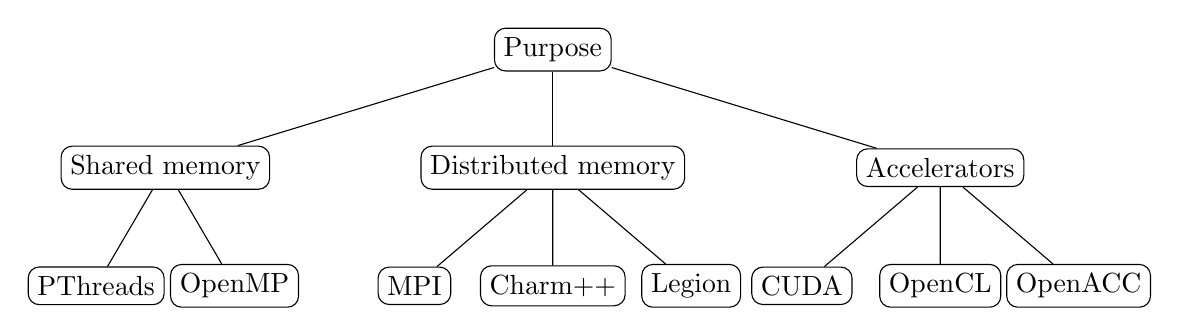
\begin{tikzpicture}[
  every node/.style = {
    level distance=1em,
    shape=rectangle, 
    rounded corners,
    draw, 
    align=center,
    top color=white%, 
   % bottom color=blue!20
  }]]
  \node {Purpose} [sibling distance=14em]
    child { node {Shared memory} [sibling distance=5em]
      child { node {PThreads}}
      child { node {OpenMP}}
    }
    child { node {Distributed memory} [sibling distance=5em]
        child{node {MPI}} 
        child{node {Charm++}}
        child{node {Legion}}
    }
    child { node {Accelerators} [sibling distance=5em]
      child {node  {CUDA}} 
      child { node {OpenCL}}
      child {node {OpenACC}}
    };
\end{tikzpicture}
\caption{Runtimes, libraries, frameworks or APIs}
\label{fig:1_HPC:software}
\end{figure}

The runtime, libraries, frameworks and APIs are summarized in figure~\ref{fig:1_HPC:software}.
They are used in combination. 
The usual one is MPI for distribution, OpenMP and CUDA to target processors and GPUs. 

%\section{Profiling tools}
%\todo{Est-ce interessant? Plus tard? Ne pas en parler?}
%\subsection{Intel suite}
%\subsection{MAQAO}
%\subsection{Allinea/MAP}

\section{Benchmarks}

All those models, theory, hardware and software leads to better understanding and characterization of machines to produce better algorithm and solve bigger and harder problems. 
The question that arise is: how to know if a machine is better than another? 
We answer that question with FLOPS, IPC, OPS or just the frequency of the machine. 
The models like BSP or law's like Amdahl and Gustafson ones propose to find the best/worst case during the execution.

In real application the only way to really know what will be the behavior of a supercomputer is to try, test real code on it. 
This is call benchmarking.
Several kind of benchmarks exists and target a specific application of supercomputers. 
We present here the most famous benchmarks of HPC and their specificities.

\subsection{TOP500}
The most famous benchmark is certainly the TOP500\footnote{http://www.top500.org}. 
It gives the ranking of the 500 most powerful, known, supercomputers of the world as its name indicates.
Since 1993 the organization assembles and maintains this list updated twice a year in June and November.

This benchmark is based on the LINPACK\cite{dongarra1994top500} a benchmark introduced by Jack J. Dongarra.
This benchmark rely on solving  dense system of linear equations. 
As specified in this document this benchmark is just one of the tools to define the performance of a supercomputer. 
It reflects "the performance of a dedicated system for solving a dense system of linear equations".
This kind of benchmark is very regular in computation giving high results for FLOPS. 

In 1965 the Intel co-fonder Gordon Moore made an observation\cite{present2000cramming} on the evolution of devices. 
He pointed the fact that the number of transistors in a dense integrated circuit doubles approximately every eighteen months.
This is know as the Moore's law. 
Looking at the last TOP500 figure presented on figure~\ref{fig:intro_top500}, in the introduction of this document, we saw that nowadays machines does not fit in the law anymore. 
This is due to the size of transistor and the energy needed to reach more powerful machines. 
The Moore's law have been sustains by the arrival of many-cores architectures such as GPU or Xeon Phi. 
Tomorrow machines architectures will have to be based on hybrid with more paradigms and tools to take part of massive parallelism.


\subsection{GREEN500}
In conjunction of the TOP500, the GREEN500\footnote{https://www.top500.org/green500/} focus on the energy consumption of supercomputers. 
The scale is based on FLOPS per watts~\cite{feng2007green500}.
Indeed the energy wall is the main limitation for next generation and exascale supercomputers. 
In the last list, November 2017, the TOP3 machines are accelerated with PEZY-SC many-core devices. 
The TOP20 supercomputers are all equipped with many-cores architectures: 5 with PEZY-SC, 14 with NVIDIA P100 and 1 with the Sunway many-core devices. 
This show clearly that the nowadays energy efficient solutions resides in many-core architecture and more than that, hybrid supercomputers. 

\subsection{GRAPH500}
The GRAPH500\footnote{https://www.graph500.org/} benchmark\cite{murphy2010introducing} focus on irregular memory accesses, and communications.
The authors try to find ways to face the futures large-scale large-data problems and data-driven analysis.
This can be see as a complement of the TOP500 for data intensive applications.
The aim is to generate a huge graph to fill all the maximum memory on the machine and then operate either:
\begin{description}
  \item[BFS:] A Breadth-First Search which is an algorithm starting from a root and exploring recursively all the neighbors. 
  This requires a lot of irregular communications and memory accesses. 
  \item[SSSP:] A Single Source Shortest Path which is an algorithm searching the shortest path from one node to the others. 
  Like the BFS it has an irregular behavior but also requires to keep more data during the computation.
\end{description}

This benchmark will be detailed in Part II Chapter II in our benchmark suite. 

\subsection{HPCG}
The High Performance Conjugate Gradient benchmark\footnote{http://www.hpcg-benchmark.org/} is a new benchmark created in 2015 and presented for the first time at SuperComputing 2015. 
The last list, November 2017 contains 115 supercomputers ranked. 
The list also offer to compare the results of Linpack compared to Conjugate Gradient. 
This benchmark is a first implementation of having both computation and 
communications aspects of HPC in the same test. 

This benchmark is presented and features:
\begin{itemize}[noitemsep,nolistsep]
\item[-] Sparse matrix-vector multiplication;
\item[-] Vector updates;
\item[-] Global dot products;
\item[-] Local symmetric Gauss-Seidel smoother;
\item[-] Sparse triangular solve (as part of the Gauss-Seidel smoother);
\item[-] Driven by multigrid preconditioned conjugate gradient algorithm that exercises the key kernels on a nested set of coarse grids;
\item[-] Reference implementation is written in C++ with MPI and OpenMP support.
\end{itemize}

\section{Conclusion}
In this chapter we presented the most used software tools for HPC. 
From inside node with shared memory paradigms, accelerators and distributed memory using message passing runtime with asynchronous or synchronous behavior. 

The tools to target accelerators architectures tend to be less architecture dependent with API like OpenMP, OpenCL or OpenACC targeting all the machines architectures. 
Unfortunately the vendor themselves have to be involve to provide the best wrapper for their architecture. 
In the mean time vendor dependent API like CUDA for NVIDIA seems to deliver the best performances.

We show through the different benchmark that hybrid architecture start to have their place even in computation heavy and communication heavy context. 
They are the opportunity to reach exascale supercomputers in horizon 2020.  



\chapter*{Conclusion}
